% Do not change document class, margins, fonts, etc.
\documentclass[a4paper,oneside,bibliography=totoc]{scrbook}

% some useful packages (add more as needed)
\usepackage[utf8]{inputenc}
\usepackage{graphicx}
\usepackage{latexsym}
\usepackage{amsmath}
\usepackage{amssymb}
\usepackage{tabularx}
\usepackage{booktabs}
\usepackage{algorithm} % you can modify the algorithm style to your liking
\counterwithin{algorithm}{chapter} % so that algorithms have chapter numbers as well
\usepackage{algorithmic}
\usepackage{csquotes}
\renewcommand{\algorithmiccomment}[1]{\hfill\textit{// #1}}
\usepackage[usenames,dvipsnames]{xcolor}
\usepackage[colorlinks,citecolor=Green]{hyperref} % you may change/remove the colors
\usepackage{lipsum} % you do not need this
\usepackage{enumitem}


% chicago citation style
\usepackage{natbib}
\bibliographystyle{chicagoa}
\setcitestyle{authoryear,round,semicolon,aysep={},yysep={,}} \let\cite\citep

% example enviroments (add more as needed)
\newtheorem{definition}{Definition} \newtheorem{proposition}{Proposition}

\begin{document}


\frontmatter \subject{Data Mining Project Report} % change to appropriate type
\title{Binary Classification of Annual Income}
\author{Miguel Mendes {\small (2179726)}, João Ferreira {\small (2179738)} \\
	\vspace{1mm}\\
	Maria Beili Mena {\small (2177377)}, Paola Tomorri {\small (2033630)}\\
	\vspace{1mm}\\
	Klea Hoxha {\small (1961755)}, Sueda Sogutlu {\small (1978962)}
  \vspace{10mm}}
  

  
\date{May 14, 2025
\vspace{10mm}}

\publishers{{\small Submitted to}\\
	\vspace{2mm}
	Prof.\ Dr.\ Sven Hertling\\
	\vspace{2mm}
	University of Mannheim\\
	\vspace{10mm}
	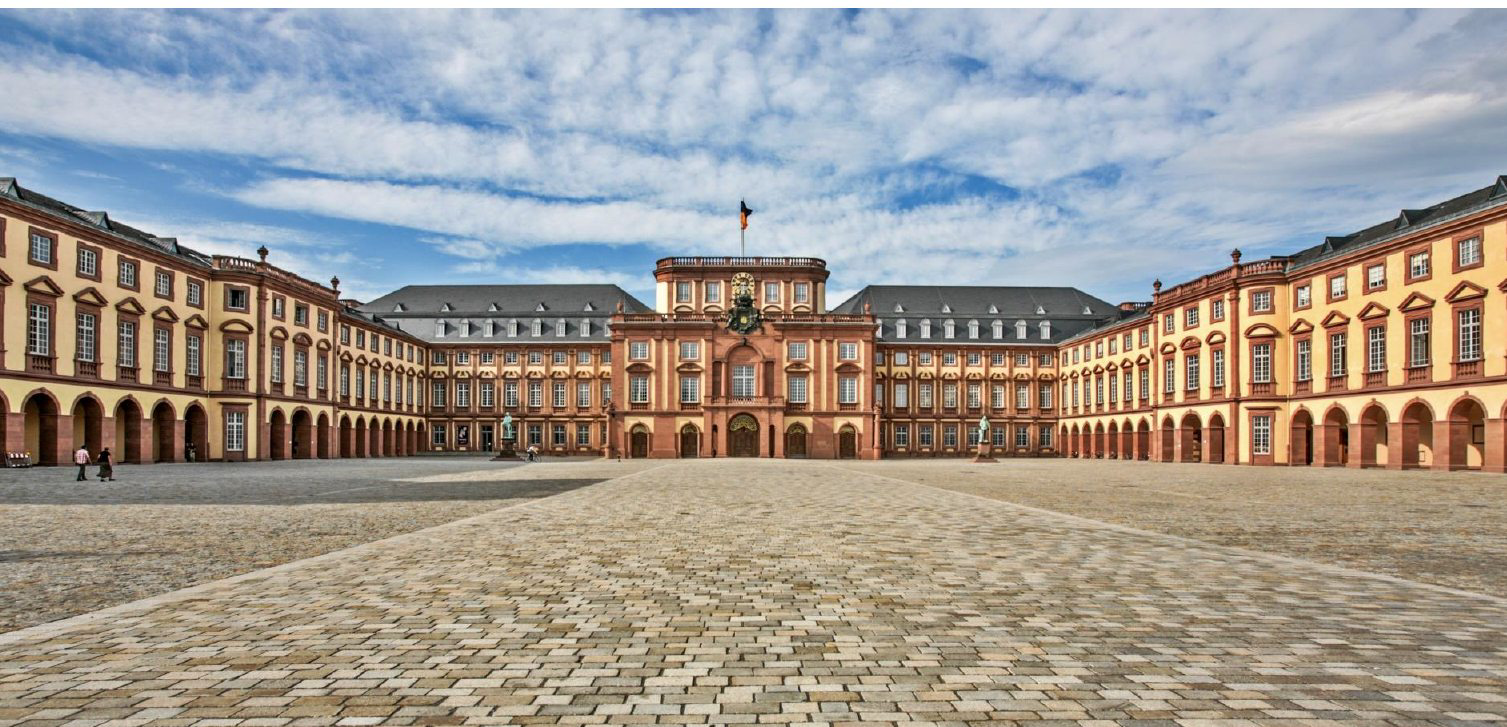
\includegraphics[width=0.9\linewidth]{screenshot024}
	}
	
\maketitle




% table of contents
%\begingroup%
%\hypersetup{hidelinks}% disable link color in TOC only
%\tableofcontents%
%\endgroup

% none of the things below is needed, but you may add them if you feel that they
% are helpful for your work \listofalgorithms \listoffigures \listoftables
% \listtheorems{definition} \listtheorems{proposition}


% okay, start new numbering ... here is where it really starts
\mainmatter

\section*{1. Application Area and Goals}
\label{ch:intro}

The aim of this project is to build a model that can predict whether a person earns more than \$50,000 a year based on different demographic and work-related features. The data comes from the 1994 U.S. Census \href{https://www.kaggle.com/datasets/anaghakp/adult-income-census}{[1]}.
This is a binary classification problem, where the target variable is income, which takes two values: $">50K"$ and "$\leq50K$". The goal of this project was to understand which features (age, education, or marital status) have the greatest influence on income level. The focus was placed on getting a stable preprocessing pipeline, improving results gradually through error analysis and trying different setups.
Understanding what influences income can also offer insights into broader socioeconomic patterns, though this project focuses on the modeling aspect.



\section*{2. Dataset Profile (Structure and Size)}

The dataset contains 31,947 entries and 12 attributes. There’s a mix of numerical and categorical data \href{https://www.kaggle.com/datasets/anaghakp/adult-income-census}{[1]}.
\subsection*{2.1 Target Variable Distribution}
One of the first observations during exploration was the class imbalance, that is, around 76\% of individuals are labelled as "$\leq50K$" (24,280 observations) and only 24\% are labelled as "$>50K$" (7,667 observations). This confirmed the need to address the imbalance in model training and evaluation.

\subsection*{2.2 Attributes Overview}
Table 1 presents a quick summary of the main features:

\begin{table}[H]
	\centering
	\fontsize{10}{12}\selectfont
	\begin{tabular}{|l|l|l|}
		\hline \textbf{Attribute} & \textbf{Type} & \textbf{Description} \\
		\hline \textit{age} & Numerical & Age in years \\
		\hline \textit{workclass} & Categorical & Type of employment \\
		\hline \textit{fnlwgt} & Numerical & Sampling weight (removed later) \\
		\hline \textit{education} & Categorical & Education level \\
		\hline \textit{education.num} & Numerical & Numeric representation of education \\
		\hline \textit{marital.status} & Categorical & Marital status \\
		\hline \textit{occupation} & Categorical & Kind of job \\
		\hline \textit{relationship} & Categorical & Family relationship \\
		\hline \textit{race} & Categorical & Ethnic group \\
		\hline \textit{sex} & Categorical & Gender \\
		\hline \textit{native.country} & Categorical & Country of origin \\
		\hline
	\end{tabular}
	\caption{Feature summary}
	\label{tab:t1}
\end{table}

The variable \textit{education.num} was kept while the variable \textit{education} was dropped, because they carry the same information. Furthermore, \textit{fnlwgt} was dropped after exploratory analysis. 

\subsection*{2.3 Data Quality: missing values and duplicates}

Three columns that used "?" as placeholders were identified: \textit{workclass} (1,772), \textit{occupation} (1,779) and \textit{native.country} (25). This results in a total of 3,576 actual missing values. In addition, 65 duplicated rows were found and removed to avoid biasing the models.

These missing values were not imputed, as they may reflect sensitive or voluntarily undisclosed information (e.g., unemployment or nationality). Instead "?" was treated as its own category, allowing the model to learn from their presence. After encoding, \textit{workclass\_nan} and \textit{occupation\_nan} showed high correlation, so \textit{workclass\_nan} was dropped to avoid redundancy. 

\subsection*{2.4 Categorical Encoding Strategy}

To encode \textit{native.country}, two strategies were explored: full one-hot encoding (adding 38 new features) and a simplified binary encoding ("USA" \textit{vs}. "non-USA"). The second approach was used to reduce dimensionality and avoid issues related to the curse of dimensionality, since most individuals were from the USA. 


\subsection*{2.5 Outliers and correlation}

Most features had reasonable value ranges. However, \textit{fnlwgt} contained extreme values and disrupted outlier detection techniques. It also showed negligible correlation with income, so it was removed.
The remaining numerical features, \textit{age} and \textit{education.num}, were kept after confirming their value ranges were reasonable.



\section*{3. Preprocessing}

To compare their effect on model performance, two parallel preprocessing pipelines were built: one using full one-hot encoding for all categorical features, and another that simplified some variables (like \textit{native.country}) to reduce dimensionality.

\subsection*{3.1 Missing Values}

As previously explained, the missing values marked as “?” were treated as valid categories instead of being imputed. This allowed the models to learn from their presence directly. 


\subsection*{3.2 Outlier Handling}

Initially, it was expected that several variables had outliers, but after thorough visual analysis, it was found that only the \textit{fnlwgt} feature was consistently problematic. As a result, it was removed from the dataset. All other numerical attributes, such as \textit{age} and \textit{education.num}, had realistic values and did not require clipping or transformation.

\subsection*{3.3 Normalization}
All numerical features (\textit{age}, \textit{education.num}) were scaled using \textit{MinMax} normalization. Since all categorical variables are One-Hot encoded, the values for all features will range between 0 and 1.

\subsection*{3.4 Feature Engineering}
No feature engineering was applied in this project, as the pre-existing variables were enough to generate solid results. Also, most of the variables were categorical, and combining them to create new variables would make them lose their meaning. If a new variable was to be created it would be Percentage of time spent studying ((\textit{education.num / age}) x 100).

\subsection*{3.5 Feature Selection}
Feature selection was based on redundancy, correlation, and multicollinearity. As a result, \textit{education}, \textit{fnlwgt}, and \textit{workclass\_nan} were dropped. Both preprocessing pipelines were used in training and compared during evaluation. 



\section*{4. Data Mining}
\subsection*{4.1 Classification models}

Multiple classification algorithms were tested to predict whether an individual’s annual income is higher or lower than 50 thousand. Furthermore, the performance of these models was evaluated and optimized through Random Searches to improve their weighted F1-score and robustness. 
Besides the baseline, which was used to set a minimum standard of performance, six basic classification models were tested:

\begin{enumerate}
	\item \textbf{Logistic Regression} – this model was chosen due to its simplicity, interpretability and efficiency. It is also proficient at handling high-dimensional data and because of its linear nature, it works well with one-hot encoding. 
	\item \textbf{Decision Tree Classifier} – this model was chosen because of its interpretability, since the tree structure shows how decisions are made based on the features. It can also capture non-linear relationships between features and doesn’t have a need for feature scaling or normalization.
	\item \textbf{Random forest} – this ensemble model was chosen because of its ability to combine multiple decision trees to improve accuracy and reduce overfitting. It is also very proficient at handling high-dimensional data and can capture complex relationships. Finally, it significantly improves model interpretation by providing feature importance.
	\item \textbf{Gradient Boosting Classifier} – this ensemble model was chosen because of its flexibility in handling various types of data (including one-hot encoded variables), its robustness to overfitting and ability to rank feature importance make it an excellent choice for real-world classification tasks.
	\item \textbf{Support Vector Classifier (SVC)} – this model was chosen because it works well in high-dimensional spaces, which is common when using one-hot encoding Additionally, SVM is less prone to overfitting, when properly tuned with regularization parameters.
	\item \textbf{Bernoulli Naïve Bayes Classifier} – this model was chosen because it assumes binary features (unlike other Naïve Bayes Algorithms), making it naturally suited for the presence/absence information in one-hot encoding. It is simple, fast, and works well when the features are conditionally independent.
\end{enumerate}

\subsection*{4.2 Hyperparameter Optimization}
After checking the performance of the models, four models stood out: Random Forest, Gradient Boosting Classifier, Support Vector Machine, and Logistic Regression. These models advanced for hyperparameter tuning, where Random Searches were used with 5-fold cross-validation to find the best combination of parameters for each model. Tables 2,3, and 4 show the parameters, their ranges, and the best combination of parameters for the three most complex models.


\begin{table}[ht]
	\centering
	\fontsize{10}{12}\selectfont
	\begin{tabular}{|l|l|l|}
		\hline \textbf{Parameter} & \textbf{Range} & \textbf{Best combination} \\
		\hline n\_estimators & 20 - 699 & 492 \\
		\hline max\_depth & 3 - 29 & 11 \\
		\hline min\_samples\_split & 2 - 29 & 4 \\
		\hline min\_samples\_leaf & 1 - 29 & 20 \\
		\hline max\_features & sqrt, log2, None & None \\
		\hline bootstrap & True, False & True \\
		\hline class\_weight & Balanced, None & None \\
		\hline
	\end{tabular}
	\caption{Parameter settings and optimization for Random Forest}
	\label{tab:t2}
\end{table}


\begin{table}[ht]
	\centering
	\fontsize{10}{12}\selectfont
	\begin{tabular}{|l|l|l|}
		\hline \textbf{Parameter} & \textbf{Range} & \textbf{Best combination} \\
		\hline n\_estimators & 50 - 999 & 574 \\
		\hline max\_depth & 2 - 19 & 4 \\
		\hline min\_samples\_split & 2 - 49 & 25 \\
		\hline mi\_samples\_leaf & 1 - 49 & 25 \\
		\hline max\_features & sqrt, log2, None, 0.3, 0.5, 0.7 & log2 \\
		\hline loss & log\_loss, exponential & log\_loss \\
		\hline subsample & 0.5 - 1.0 & 0.54079 \\
		\hline learning\_rate & 0.001 - 0.3 & 0.08907 \\
		\hline
	\end{tabular}
	\caption{Parameter settings and optimization for Gradient Boosting Classifier}
	\label{tab:t3}
\end{table}

\begin{table}[H]
	\centering
	\fontsize{10}{12}\selectfont
	\begin{tabular}{|l|l|l|}
		\hline \textbf{Parameter} & \textbf{Range} & \textbf{Best combination} \\
		\hline C & 0.01 - 1000 & 342.93686 \\
		\hline kernel & rbf, linear, poly, sigmoid & rbf \\
		\hline gamma & 1e-5, 1e-2 & 0.00962 \\
		\hline degree & 2 - 5 & 4 \\
		\hline coef0 & 0 - 1 & 0.67910 \\
		\hline shrinking & True, False & True \\
		\hline class weight & None, balanced & None \\
		\hline tol & 1e-5, 1e-2 & 0.00737 \\
		\hline max iter & -1, 19999 & 6370 \\
		\hline
	\end{tabular}
	\caption{Parameter settings and optimization for SVC}
	\label{tab:t4}
\end{table}

As previously discussed in the preprocessing phase, two different approaches were used to prepare the data. For both approaches, the models selected for training were the same. Additionally, the results obtained from the second approach (approach with half the variables) were almost identical to those of the first approach (except Bernoulli Naive Bayes in the train weighted F1-score, where it was 0.78 and now is 0.77). Thus, it is possible to assume that the dataset does not suffer from the curse of dimensionality. 

Finally, since the results were so identical, there is no need to perform random searches on all the models, and the best model for both approaches is the Gradient Boosting Classifier. With this said, a random search with the same optimized parameters was still performed for the best model to prove that there is no curse of dimensionality. The random search results of the Gradient Boosting Classifier for both approaches were identical, confirming no dimensionality curse.



\section*{5. Evaluation}

\subsection*{5.1 Evaluation Setup}

Before evaluating the models' performance, the dataset was divided into training (60\%), validation (20\%), and test (20\%) sets. This split was stratified to ensure the same distribution of target classes in all the subsets. To avoid data leakage, all preprocessing steps were only fit to the training data. For the hyperparameter tuning, 5-fold cross-validation was employed, balancing computational efficiency and performance reliability. 

After identifying the best combinations of parameters for each Random Search, each model is evaluated on the validation set. Until this point, the test set remains untouched, and only now is it used to assess the best-performing models. Considering class imbalance, the weighted F1-score is used to evaluate performance for all models. This metric was chosen for many reasons, such as: it balances precision and recall, accounting for class frequency; It also generates a more relevant overall score by calculating the F1-score of both target classes and weighing them by the real number of observations; Finally, it does not get inflated by the majority class making it more reliable when there is class dominance. 

This evaluation setup ensures that the results are unbiased and avoid complications such as overfitting or data leakage, by applying proper data splitting and evaluation metrics. 

\subsection*{5.2 Discussion of Results}

The evaluation process began by using a baseline, namely a Dummy Classifier, to predict the most frequent class. The purpose of this baseline was to create a minimal standard of performance. Therefore, any relevant model would be capable of outperforming the baseline. The following step compares the validation results between models to see which models deserve to advance for hyperparameter tuning. The best models were selected based on factors such as performance (see Table 5), overfitting, and number of hyperparameters. Out of all the basic classification models, these were the best ones:


\begin{itemize}
	\item \textbf{Random Forest} – good performance but has some overfit. Nonetheless, it has potential for improvement. 
	\item \textbf{Gradient Boosting Classifier} – best overall score.
	\item \textbf{Support Vector Classifier} (SVC) – second best performer tied with logistic regression. It doesn’t overfit and shows space for improvement considering it scored higher on the validation than on the training set. 
	\item \textbf{Logistic Regression} – despite not having a lot of parameters to test, and consequently, little space for improvement, the model achieved good results in the basic model and was given a chance for further improvement.
\end{itemize}

Other models did not perform as well and were not selected for hyperparameter tuning:
\begin{itemize}
	\item \textbf{Decision Tree} - exhibited similar results to random forest, but the former were slightly lower which led to choosing random forest as the best model between the two. 
	\item \textbf{Bernoulli Naïve Bayes Classifier} - was outperformed by all the other models, therefore it wasn’t a good choice for further improvement.
\end{itemize} 

\begin{table}[H]
	\centering
	\fontsize{10}{12}\selectfont
	\begin{tabular}{|l|l|l|}
		\hline \textbf{Model} & \textbf{Train F1-Score} & \textbf{Validation F1-Score} \\
		\hline Logistic Regression & 0.83 & 0.83 \\
		\hline Decision Tree & 0.95 & 0.79 \\
		\hline Random Forest & 0.95 & 0.81 \\
		\hline Gradient Boosting & 0.84 & 0.84 \\
		\hline SVM & 0.82 & 0.83 \\
		\hline BernoulliNB & 0.77 & 0.76 \\
		\hline
	\end{tabular}
	\caption{Values for basic classification models}
	\label{tab:t5}
\end{table}


After hyperparameter optimization (Table 6), the Random Forest and Gradient Boosting models obtained the best validation and training set results. However, these scores are not too far from the other two models, as all models converged around the same limit. This happens because all the random searches had a big search space and could not produce better values than these. Therefore, for the dataset in question, 0.84 is probably the limit that can be achieved. After further investigation, the Gradient Boosting Classifier produced a slightly better result and was selected as the best model.

\begin{table}[ht]
	\centering
	\fontsize{10}{12}\selectfont
	\begin{tabular}{|l|l|l|}
		\hline \textbf{Model} & \textbf{Train F1-Score} & \textbf{Validation F1-Score} \\
		\hline Random Forest & 0.84 & 0.84 \\
		\hline Gradient Boosting & 0.84 & 0.84 \\
		\hline SVC & 0.83 & 0.83 \\
		\hline Logistic Regression & 0.83 & 0.83 \\
		\hline 
	\end{tabular}
	\caption{Values after hyperparameter optimization}
	\label{tab:t6}
\end{table}

\subsection*{5.3 Error Analysis of the best model – Gradient Boosting Classifier}

Plots were constructed to understand the best model’s predictive capabilities and error
patterns. Despite the strong performance of the Gradient Boosting model, some errors
were noticed. Overall, the model shows predictive limitations in 6 out of 203 categories
(the joint analysis of two variables), showing an error rate greater than 35\%. The three
combinations of variables the model struggles the most with are:
 

\begin{itemize}
	\item Prof-specialty as occupation and more than 60 years old (43\%) – Figure 1
	\item Married with Armed Forces spouse between ages 40 and 60 (100\%) – Figure 2 
	\item Wives who work as an adm-clerical or in transport-moving (40\% each) – Figure 3
\end{itemize}


\begin{figure}[H]
	\centering
	\includegraphics[width=0.8\linewidth]{"../../../../(Sem assunto)/Occupation_vs_Age_group"}
	\caption{Error rate by Occupation and Age Group}
	\label{fig:occupationvsagegroup}
\end{figure}

\begin{figure}[H]
	\centering
	\includegraphics[width=0.6\linewidth]{"../../../../(Sem assunto)/Age_group_vs_marital_status"}
	\caption{Error rate by Age Group and Marital Status}
	\label{fig:agegroupvsmaritalstatus}
\end{figure}


\begin{figure}[H]
	\centering
	\includegraphics[width=0.7\linewidth]{"../../../../(Sem assunto)/Occupation_vs_Realtionship"}
	\caption{Error Rate by Occupation and Relationship}
	\label{fig:occupationvsrealtionship}
\end{figure}



\section*{5.4 Feature Importance}

The Random Forest model (which yielded one of the best results) was used to determine which features had a higher impact on the results. Furthermore, this model already includes the Gini impurity metric, facilitating feature importance analysis. In Figure 4, the most influential variable in reducing Gini impurity is \textit{marital.status Married-civ-spouse} (people who are married to a civilian). There are also two other meaningful variables regarding Gini impurity reduction, the \textit{education.num} (number of years studied) and age. All other variables yielded low values of Gini impurity reduction.



\begin{figure}[H]
	\centering
	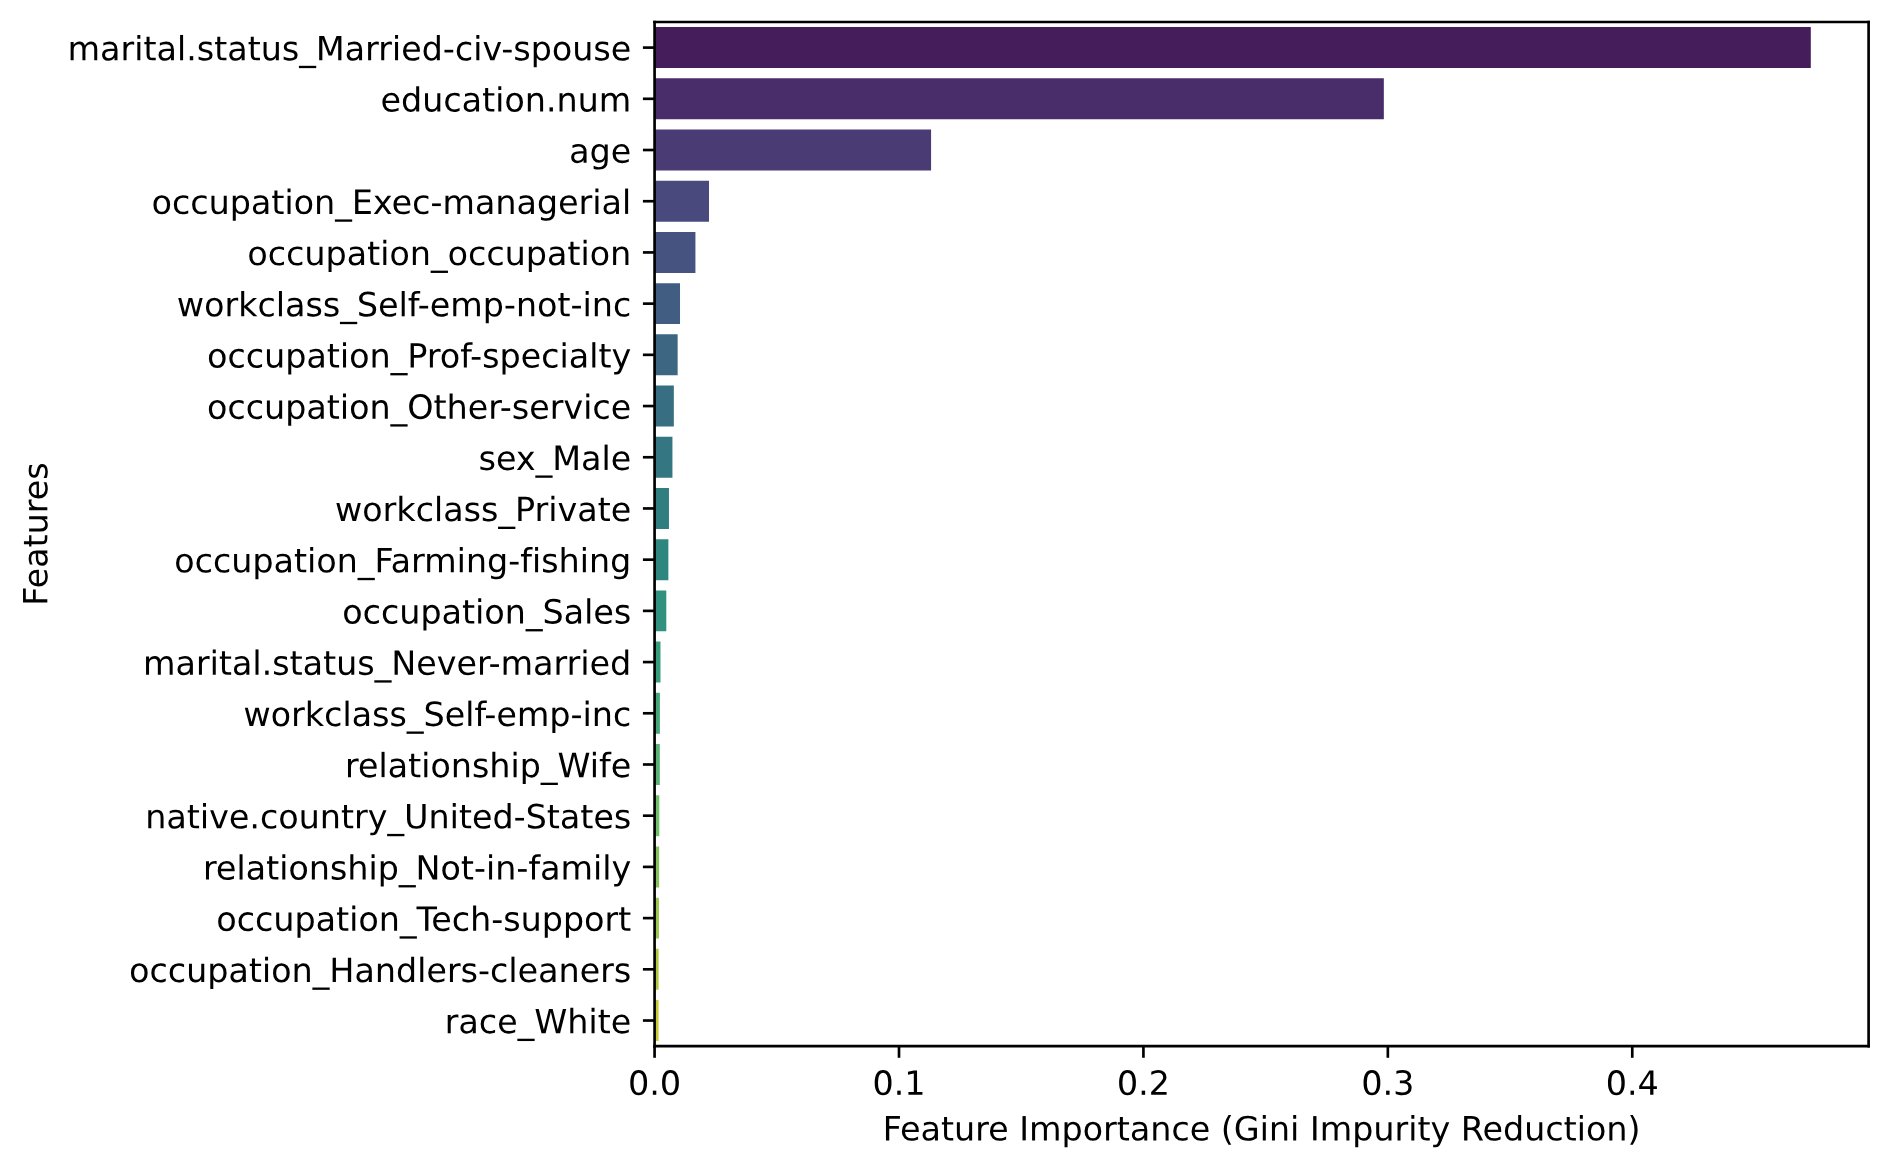
\includegraphics[width=0.6\linewidth]{screenshot023}
	\caption{Top 20 most influential features (Random Forest)}
	\label{fig:screenshot023}
\end{figure}

Overall, these three variables are the most important ones in predicting if the annual income of an individual is higher or lower than 50K.

\subsection*{5.5 Comparison of state-of-the-art results}

The results from the best model were compared to those present in Kaggle to understand better how well our model was performing. This comparison shows that our model produces better results than 88\% of the other users’ models (out of 9 models, eight were worse, and the weighted F1-score for these models ranged between 0.5962 and 0.82), which means that there was only 1 model that outperformed ours, getting a weighted F1-score of 0.89 \href{https://www.kaggle.com/code/thotasivateja57/accuracy-approximately-90-percent}{[2]}.  However, to get this result, the user encoded each variable with the frequency of each category. This approach was not followed, as it could be problematic by preventing the model from learning the difference between two categories with the same frequency.  


\section*{6. Results}

In the project's final phase, the final predictions were made on the test data, which had been left untouched. The model to be tested was the best from the evaluation phase, the Gradient Boosting (GB) Classifier. The classification report (Table 7) shows that results obtained in the test set are very similar to those obtained on the train and validation subsets, as expected, since there was no overfit. It also indicates that the model achieved very good values for the majority class (income $\leq$ 50K) and satisfactory results for the minority class (income $>$ 50K). Furthermore, the weighted F1-score obtained was 0.84, meaning the model has good generalization and predictive performance. Overall, the model is assumed to be trustworthy and generates more than satisfactory results in unseen data. Compared to the Dummy Classifier baseline, this model overwhelmingly outperformed the baseline in almost all metrics. For instance, the weighted F1-score for the baseline was 0.66, a value much lower than the GB Classifier, which was 0.84. 
\begin{table}[h]
	\centering
	\fontsize{9}{12}\selectfont
	\begin{tabular}{|l|l|l|l|l|}
		\hline \multicolumn{3}{|c|}{\textbf{Gradient Boosting Optimized Classification Report}} & &  \\
		\hline & precision & recall & f1-score & support \\
		\hline 0 & 0.88 & 0.92 & 0.90 & 4842 \\
		\hline 1 & 0.70 & 0.59 & 0.64 & 1535 \\
		\hline accuracy & & & 0.84 & 6377 \\
		\hline macro avg & 0.79 & 0.76 & 0.77 & 6377 \\
		\hline weighted avg & 0.83 & 0.84 & 0.84 & 6377 \\
		\hline
	\end{tabular}
	\caption{Gradient Boosting Classification}
	\label{tab:t7}
\end{table}

Additionally, the baseline could only predict the majority class, obtaining an F1-score of 0 for the minority class. This problem does not happen with the GB Classifier, as seen in Figure 6, where the F1-score for the minority class is 0.64. 

To further understand the predictive capabilities and errors made by the Gradient Boosting Classifier, a confusion matrix was developed:

\begin{figure}[H]
	\centering
	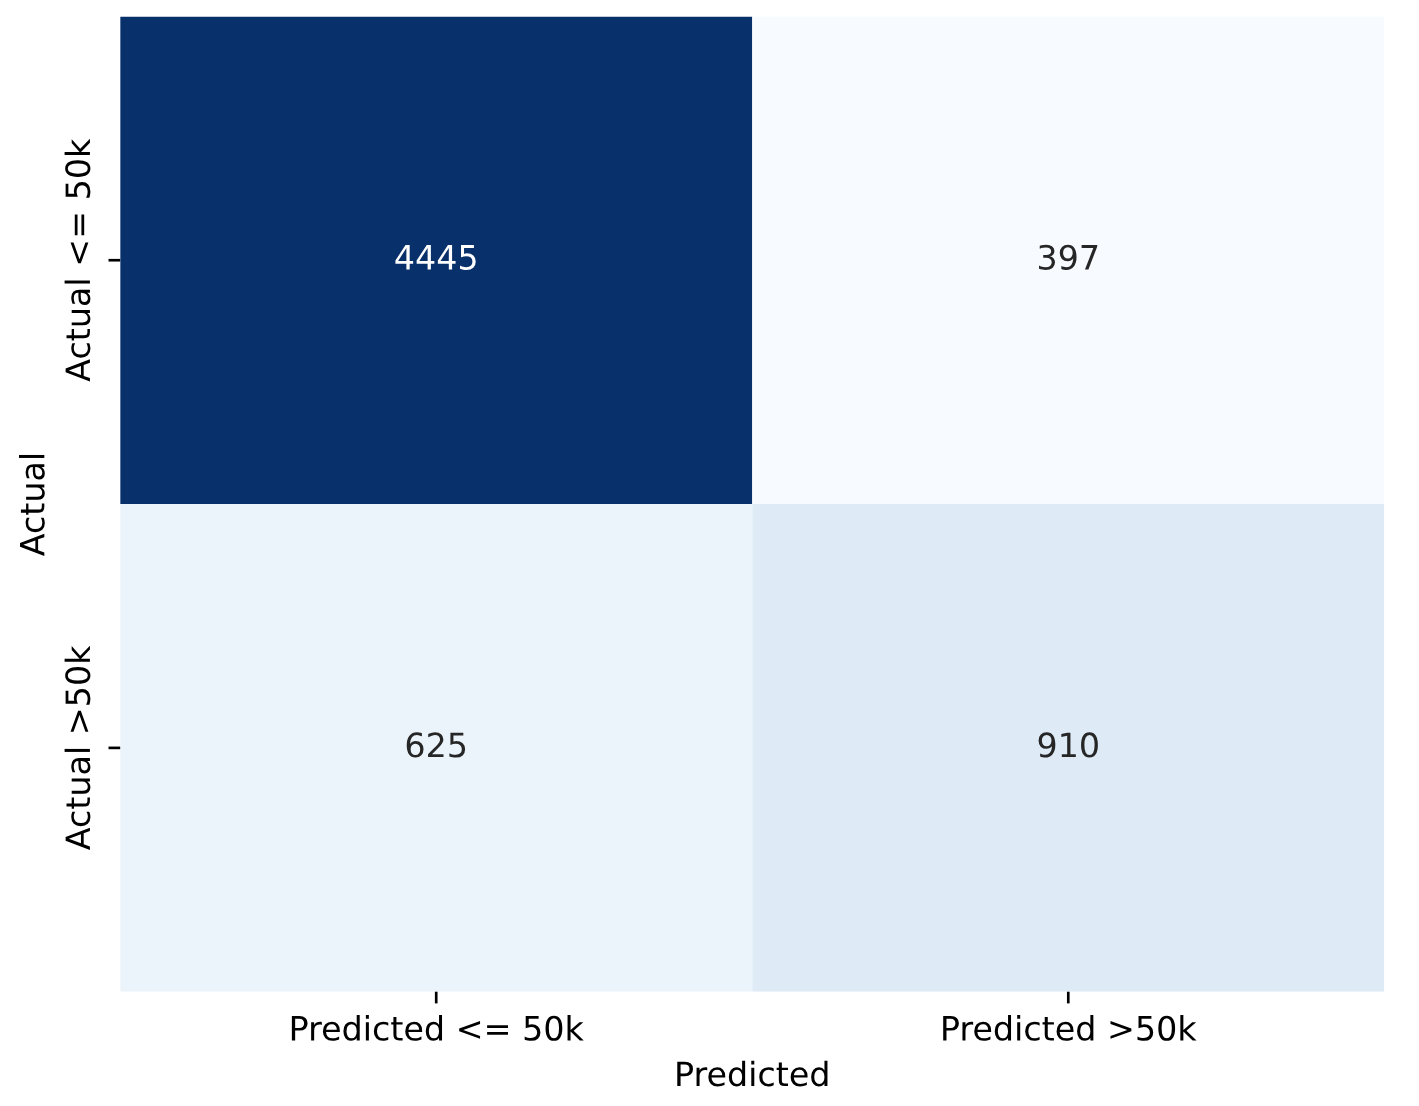
\includegraphics[width=0.5\linewidth]{screenshot020}
	\caption{Confusion matrix for Gradient Boosting Classifier}
	\label{fig:screenshot020}
\end{figure}

Figure 5 shows that the model is more effective at predicting lower income individuals (income $\leq$ 50K), correctly predicting 4445 out of 4842 low-income cases. On the other hand, the model struggles with predicting high-income individuals (income $>$ 50K), considering it failed to predict them 625 times. Furthermore, out of 1535 high-income cases, the model only correctly predicted 910. This means that it misclassified 40\% of high-income cases. Given the problem itself – predicting if an individual earns more or less than 50 thousand yearly – the model is much more successful at predicting low-income individuals. This can be useful for problems such as identifying individuals who qualify for social benefits or identifying students from poorer backgrounds eligible for student grants, among many other uses. On the other hand, this project may not be as helpful for cases where the misclassification of high-income individuals is crucial. For instance, granting exclusive membership programs or filtering individuals eligible for loans.

\newpage

\section*{Bibliography}


\begin{enumerate}[label={[}\arabic*{]}.]
	\item https://www.kaggle.com/datasets/anaghakp/adult-income-census
	\item https://www.kaggle.com/code/thotasivateja57/accuracy-approximately-90-percent
\end{enumerate} 


\section*{Declaration of Used AI Tools}

\begin{tabular}{|l|l|l|l|l|l|l|l|}
	\hline Grammarly & Text correction &  Throughout &  ++  \\
	\hline ChatGPT & Summarization &  Throughout &  -   \\
	\hline ChatGPT & Hyperparameter search suggestion &  Section 4.2 & +  \\
	\hline
\end{tabular}


\end{document}
